% 第01章 计算机系统全貌与学习路线
% 由 scripts/new-chapter.py 生成。
% 单章预览：scripts/build.sh chapters/01-system-overview/chapter.tex
%
% 素材约定（路径都相对本章目录）：
%   本节专属的图   figures/<节文件名>/xxx     代码  code/<节文件名>/xxx
%   本章多节共用   figures/xxx                代码  code/xxx
%   跨章复用       放在主用它的那一章，其他章用 ../NN-xxx/figures/xxx 引用
\documentclass[../../main.tex]{subfiles}

\begin{document}

\chapter{计算机系统全貌与学习路线}
\label{ch:01-system-overview}
\section{为什么软硬件要一起学}
\label{sec:01-system-overview-01}

本节要回答的核心问题是：一段程序究竟是怎样一步步变成硬件上的动作的？
理解这条链路，是后面每一章能够“接着往下搭”的前提。硬件与软件的分工
可参考经典教材\citep{patterson2020}。

本节与后续各章共用同一条主线：同一条指令、同一颗处理器核、同一块开发板，
每一章只在这个系统上增加一层能力。

\begin{figure}[htbp]
\centering
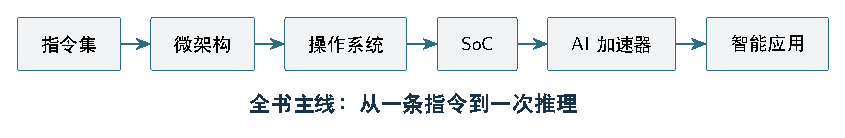
\includegraphics[width=.96\linewidth]{figures/system-stack}
\caption{全书主线：从一条指令到一次推理}
\label{fig:system-stack}
\end{figure}

\begin{definition}[指令集架构]
指令集架构（ISA）是软件与硬件之间的契约，规定了可见的寄存器、指令语义、
数据类型与异常行为；它不规定这些行为由怎样的电路实现。
\end{definition}

% TODO：撰写本节正文。建议结构：
%   1) 问题引入与学习目标
%   2) 原理与机制（配图、公式）
%   3) 示例或实验步骤
%   4) 小结与思考题
本节待撰写。为便于分工，正文请按“概念—机制—示例”的顺序展开，
并在每小节末尾留出一段可以动手验证的实验说明。

\section{我们的组织}
\label{sec:01-system-overview-02}

% TODO：撰写本节正文。建议结构：
%   1) 问题引入与学习目标
%   2) 原理与机制（配图、公式）
%   3) 示例或实验步骤
%   4) 小结与思考题
本节待撰写。

\section{与我们对接的竞赛}
\label{sec:01-system-overview-03}

% TODO：撰写本节正文。建议结构：
%   1) 问题引入与学习目标
%   2) 原理与机制（配图、公式）
%   3) 示例或实验步骤
%   4) 小结与思考题
本节待撰写。

\section{本书编排总览}
\label{sec:01-system-overview-04}

% TODO：撰写本节正文。建议结构：
%   1) 问题引入与学习目标
%   2) 原理与机制（配图、公式）
%   3) 示例或实验步骤
%   4) 小结与思考题
本节待撰写。

\section{大学四年学习建议}
\label{sec:01-system-overview-05}

四年路线按"同一条主线逐层加码"组织：每一年都在同一个系统上增加一层能力，
而不是换一个互不相关的题目。示意安排见\cref{tab:roadmap}。

\begin{table}[htbp]
\centering
\caption{四年学习路线示意}
\label{tab:roadmap}
\begin{tabularx}{\linewidth}{@{}P{14mm}P{40mm}Y@{}}
\toprule
学年 & 主线 & 可验收的产物 \\
\midrule
大一 & 数字逻辑与计算机组成 & 用硬件描述语言实现单周期处理器，仿真跑通一段汇编 \\
大二 & 指令集与微架构 & 五级流水线上板运行，正确处理冒险与旁路 \\
大三 & 工具链与操作系统 & 在自研处理器核上启动实时操作系统或精简 Linux \\
大四 & SoC 与智能应用 & 在自研加速器上跑通量化模型的 TinyML 推理 \\
\bottomrule
\end{tabularx}
\end{table}

% TODO：撰写本节正文。建议结构：
%   1) 问题引入与学习目标
%   2) 原理与机制（配图、公式）
%   3) 示例或实验步骤
%   4) 小结与思考题
本节待撰写。


\end{document}
